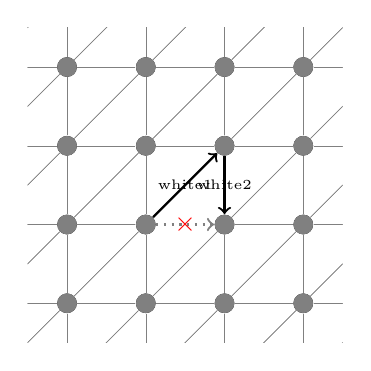
\begin{tikzpicture}
	
	%\clip (2.25cm,-0.5cm) rectangle +(3.25cm,3.0cm);
	\clip (2.5cm,1.5cm) rectangle +(4cm,4cm);
	
	\begin{scope}[minimum size=0.25cm,inner sep=0]
		\foreach \y in {-1,...,8}{
			\foreach \x in {-1,...,8}{
				\ifthenelse{\equal{\x\y}{43} \OR \equal{\x\y}{54} \OR \equal{\x\y}{53}}{
					\node (chip \x \y) at (\x,\y) [fill,circle] {};
				}{
					\node (chip \x \y) at (\x,\y) [fill=gray,circle] {};
				}
			}
		}
	\end{scope}
	
	\begin{scope}[help lines]
		\foreach \y in {0,...,7}{
			\foreach \x in {0,...,7}{
				\pgfmathtruncatemacro{\xx}{\x+1}
				\pgfmathtruncatemacro{\yy}{\y+1}
				\draw (chip \x \y) -- (chip \xx \yy);
				
				\pgfmathtruncatemacro{\xx}{\x-1}
				\pgfmathtruncatemacro{\yy}{\y-1}
				\draw (chip \x \y) -- (chip \xx \yy);
				
				\pgfmathtruncatemacro{\xx}{\x+1}
				\pgfmathtruncatemacro{\yy}{\y+0}
				\draw (chip \x \y) -- (chip \xx \yy);
				
				\pgfmathtruncatemacro{\xx}{\x-1}
				\pgfmathtruncatemacro{\yy}{\y+0}
				\draw (chip \x \y) -- (chip \xx \yy);
				
				\pgfmathtruncatemacro{\xx}{\x+0}
				\pgfmathtruncatemacro{\yy}{\y+1}
				\draw (chip \x \y) -- (chip \xx \yy);
				
				\pgfmathtruncatemacro{\xx}{\x+0}
				\pgfmathtruncatemacro{\yy}{\y-1}
				\draw (chip \x \y) -- (chip \xx \yy);
			}
		}
	\end{scope}
	
	% Hide existing link and redraw as dead link
	\draw [ultra thick, white] (chip 43) -- (chip 53);
	\draw [->, gray, thick, dotted]
	      (chip 43)
	   -- coordinate (dead link center)
	      (chip 53);
	\node [red] at (dead link center) {$\times$};
	
	% Draw emergency route 1
	\draw [ultra thick, white] (chip 43) -- (chip 54);
	\draw [->, thick]
	      (chip 43)
	   -- coordinate (first link center)
	      (chip 54);
	\node [font=\tiny] at (first link center) {\contour{white}{1}};
	
	% Draw emergency route 2
	\draw [ultra thick, white] (chip 54) -- (chip 53);
	\draw [->, thick]
	      (chip 54)
	   -- coordinate (second link center)
	      (chip 53);
	\node [font=\tiny] at (second link center) {\contour{white}{2}};
	
\end{tikzpicture}

